\section{Community Engagement}
\label{sec:community}

The St.~Louis region is well known for its strength in plant sciences.
At the geographic center of the regional AgTech innovation corridor is
39~North, an innovation district in St.~Louis County that includes Bayer AG's
US Crop Science headquarters, the Donald Danforth Plant Science Center,
startup incubators, and many businesses with a technology focus
(see Figure~\ref{fig:39N}).

\begin{figure}[ht]
\centering
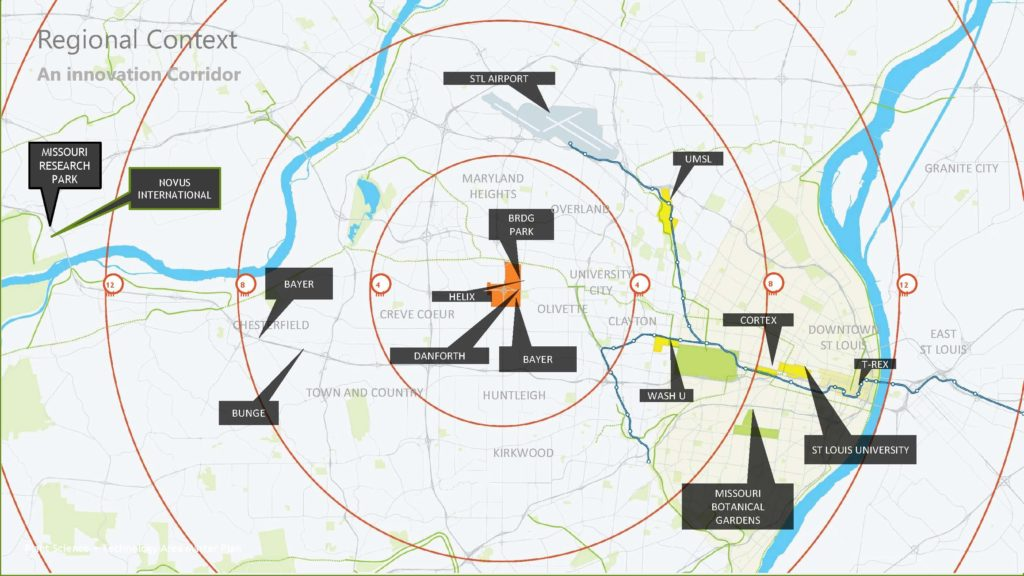
\includegraphics[width=0.75\linewidth]{figures/39N}
\caption{39 North is in the center of a regional AgTech innovation corridor.}
\label{fig:39N}
\end{figure}

We have current connections with the Donald Danforth Plant Science
Center (a collaborating organization) and two commercial firms
located in 39~North,
VelociData, Inc.\footnote{\url{http://www.velocidata.com}} and
BECS Technology, Inc.\footnote{\url{http://www.becs.com}}
These three organizations have agreed to help us with prototype deployment
and assessment.
We are also engaging with the St.~Louis Economic Development Partnership,
the economic development team serving St.~Louis City and County.
All four organizations have agreed to work with us in
developing a relationship with the 39~North community.
Another approach we will use towards community engagement is to participate
in Venture Caf\'e\footnote{\url{http://vencafstl.org}}, which gathers once per
month in 39~North (in addition to its weekly gatherings in midtown St.~Louis).
